% ---------------------------------------------------
%
% Trabajo de Fin de Grado. 
% Author: Laura Padrón Jorge. 
% Capítulo: Tecnologías utilizadas en el Trabajo de Fin de Grado. 
% Fichero: Cap2_Technology.tex
%
% ----------------------------------------------------
%

\cleardoublepage
\chapter{Herramientas y Tecnologías utilizadas} \label{chap:Tecnologias} 

Este capítulo tiene como objetivo presentar las distintas herramientas software y tecnologías empleadas por la alumna en el desarrollo de su TFG.

\section{Herramientas de Desarrollo}

A continuación se explicarán brevemente las distintas herramientas software utilizadas en el proyecto. 

\subsection{Android Studio}

Android Studio \cite{URL::AndroidStudio} es el IDE (Entorno de Desarrollo Integrado) oficial para el desarrollo de aplicaciones en Android, basado en IntelliJ IDEA \cite{URL::IntelliJIDEA}. Android Studio ofrece una serie de funcionalidades que han facilitado a la desarrolladora numerosas tareas, entre ellas podemos destacar:


\begin{itemize}
\item Un sistema de compilación basado en Gradle\cite{URL::Gradle} que ha simplificado tanto la inserción de dependencias de las distintas librerías que se han tenido que utilizar, como la compilación de la aplicación.
\item Un emulador rápido y fácil de utilizar que ha ayudado a visualizar las distintas pantallas durante el desarollo aunque no ha sido de mucha utilidad para probar el funcionamiento al ser dependiente la app de la tecnología Bluetooth.
\item La facilidad para publicar cambios a aplicaciones ya funcionando sin tener que eliminar y volver a crear un nuevo APK parando la app.
\item Un sistema de visualización de las diferentes pantallas muy completo, con soporte visual para añadir componentes y cambiar atributos fácilmente.
\item Un sistema de depuración, con una interfaz sencilla e intuitiva.
\end{itemize} 

\begin{figure}[h]
	\centering
	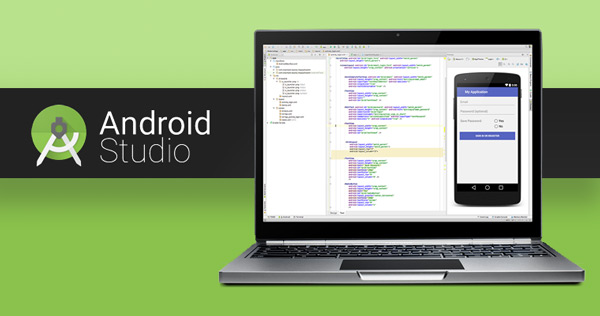
\includegraphics[width=\columnwidth]{androidstudio}
	\caption{Android studio, un IDE flexible e intuitivo.}
	\label{fig:androidstudio}
\end{figure}

Se ha utilizado este IDE frente a otros como Eclipse + ADT \cite{URL::eclipseADT} debido a que en la actualidad es el IDE oficial con soporte de Google. Se ha preferido aprender a utilizar este entorno con vistas al futuro, ya que parece que se consolidará como el preferido para los desarrolladores Android.

\subsection{LaTex}

LaTeX \cite{URL::LaTeX} es un sistema de composición de textos, orientado a la creación de documentos que presenten una alta calidad tipográfica. Por sus características y posibilidades, es usado especialmente en la generación de artículos y libros científicos que incluyen, entre otros elementos, expresiones matemáticas, gráficos o figuras.


LaTeX está formado por un gran conjunto de macros de TeX, escrito por Leslie Lamport en 1984, con la intención de facilitar el uso del lenguaje de composición tipográfica, creado por Donald Knuth. LaTeX es software libre bajo licencia LPPL.


Se ha decidido utilizar este sistema debido al carácter profesional que le aporta a los documentos. Ha sido una buena oportunidad para aprender a usar un sistema de composición de texto como este, ya que en un futuro puede ser beneficioso el saber manejar esta herramienta. 


Si bien es cierto, que el uso de esta herramienta frente a otros editores más familiares ha sido algo tedioso en el inicio, es verdad que una vez acostumbrada a utilizarla ha resultado ser múy eficaz. En el proceso de aprendizaje se recurrió principalmente a manuales por internet, alguno a destacar en español sería:  \cite{URL::manualLatex}

\subsection{Github}

GitHub es una forja (plataforma de desarrollo colaborativo) para alojar proyectos utilizando el sistema de control de versiones Git. Utiliza el framework Ruby on Rails por GitHub, Inc. (anteriormente conocida como Logical Awesome). Desde enero de 2010, GitHub opera bajo el nombre de GitHub, Inc. El código se almacena de forma pública, aunque también se puede hacer de forma privada, creando una cuenta de pago.


Se ha decidido crear un repositorio en esta plataforma para poder llevar un control y una trazabilidad del proyecto. El tutor y la alumna han trabajado en este repositorio de manera conjunta. En el caso del tutor, principalmente para revisar el seguimiento semanal y llevar un control de las tareas. En el caso de la alumna, para tener un repositorio donde subir los distintos elementos que se han ido generando a lo largo del trabajo. Aparte de este repositorio, también se ha abierto un segundo repositorio asociado a la OSL para subir el código una vez terminado como parte del Programa de Apoyo a Trabajos Finales Libres (PATFL) \cite{URL::PATFL} de la ULL. Accesible libremente desde: \cite{URL::repositorioAplicacion}


Mediante el uso de este repositorio, la alumna ha conseguido ampliar sus conocimientos en Git y familiarizarse con la interfaz de GitHub. Previamente se había utilizado como repositorios GitLab, SVN y RTC en otros proyectos, por lo que no ha sido una complicación mayor utilizar este sistema.


\begin{figure}[h]
	\centering
	
\includegraphics[width=\columnwidth]{github}
	\caption{La plataforma de desarrollo colaborativo GitHub.}
	\label{fig:github}
\end{figure}

\section{Tecnologías utilizadas}

A continuación se explicarán las distintas tecnologías utilizadas en el desarrollo de la aplicación.

\subsection{El Sistema Operativo Android}

Android es un sistema operativo que emplea Linux en la interfaz del hardware.  Los componentes del S.O subyacentes se codifican en C o C++ pero las aplicaciones se desarrollan en Java. De esta manera Android asegura una amplia operatividad en una gran variedad de dispositivos debido a dos hechos: la interfaz en Linux ofrece gran potencia y funcionalidad para aprovechar el hardware, mientras que el desarrollo de las aplicaciones en Java permite que Android sea accesible para un gran número de programadores conocedores del código.

Este S.O fue diseñado principalmente para dispositivos móviles con pantalla táctil: smartphones, tablets y otros dispositivos como televisores o automóviles. Fue desarrollado inicialmente por Android Inc., empresa que fue respaldada económicamente por Google y más tarde comprada por esta misma empresa.

Actualmente tiene una gran comunidad de desarrolladores creando aplicaciones para extender la funcionalidad de los dispositivos. A fecha de hoy existen más de un millón de aplicaciones disponibles para la tienda oficial de Apps de Android: Google Play \cite{URL::GooglePlay} sin tener en cuenta las aplicaciones de otras tiendas no oficiales, como por ejemplo, la tienda de aplicaciones de Samsung Apps \cite{URL::SamsungApps}.

\subsection{Los Beacons}

Los \textit{''Beacons''} \cite{URL::Beacon}, cuya traducción del inglés equivaldría a \textit{'balizas'} o \textit{'faros'}, son una tecnología emergente que desde algunos años se intenta abrir paso en el mercado. Como su propio nombre indica, estos dispositivos intentan ser un mecanismo de guía, dando una solución al posicionamiento en interiores, donde otras tecnologías, como el GPS o el Wifi dejan de funcionar o resultan imprecisas. Sin embargo, estos no son los únicos usos de los beacons, actualmente muchas empresas están ampliando sus usos a otros campos.


A continuación se intentará responder a las preguntas más frecuentes que nos pueden surgir con respecto a esta tecnología:


\begin{itemize}
\item ¿Qué es un Beacon?
\item ¿Cómo funcionan estos dispositivos?
\item ¿Qué rango de alcance poseen?
\item ¿Con qué dispositivos móviles son compatibles? 
\item ¿Qué ventajas y desventajas tienen con respecto a otras tecnologías?
\item ¿Qué usos se le ha dado a esta tecnología hasta ahora?
\end{itemize}

\begin{figure}[!h]
        \begin{floatrow}
        \ffigbox{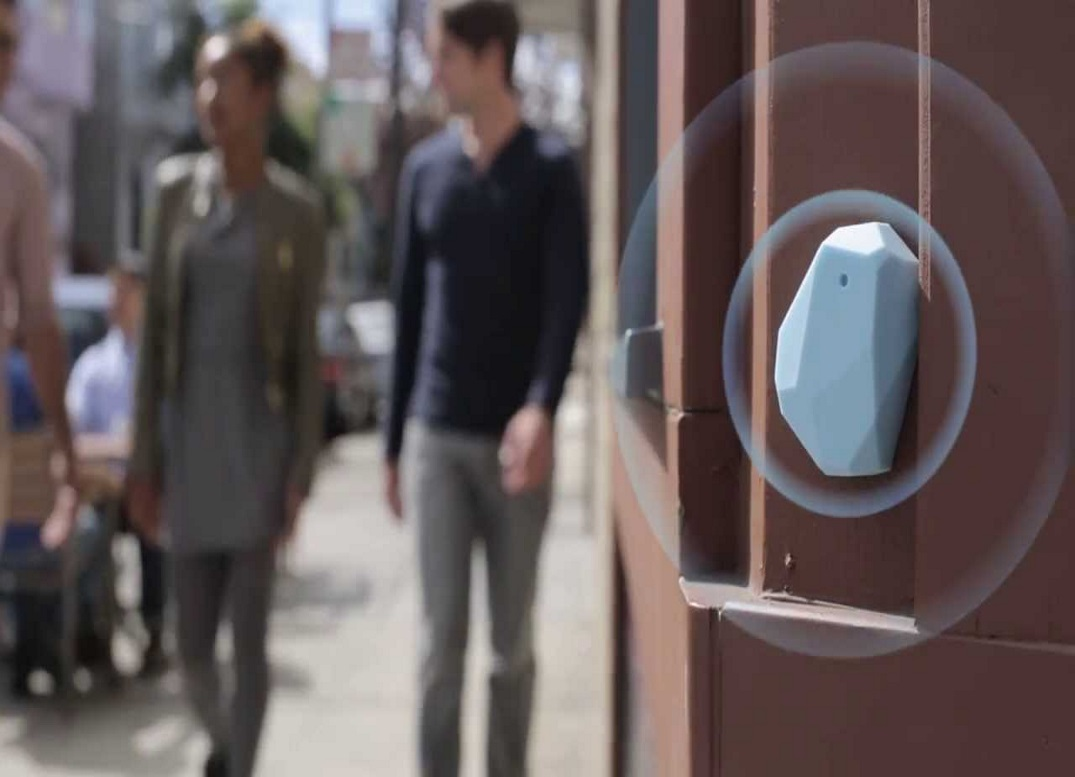
\includegraphics[width=\textwidth/2]{estimoteBeacon}}{\caption{Uno de los beacons de la compañia Estimote}\label{fig:estimote_Beacon}}
        \ffigbox{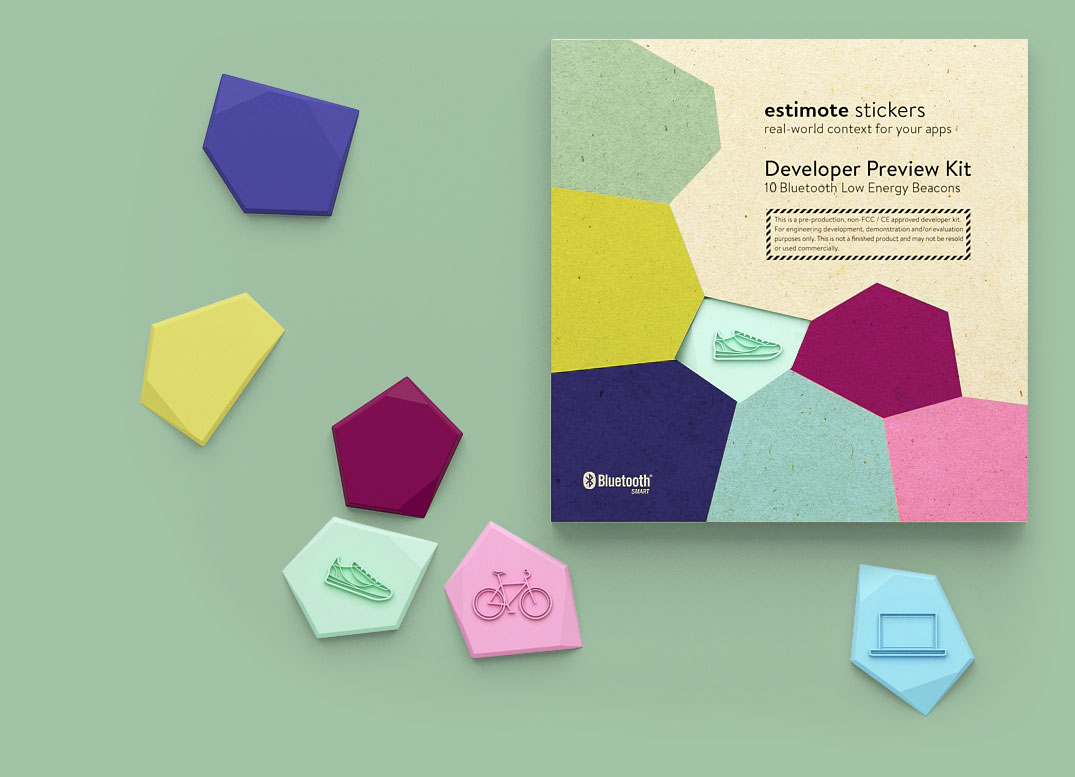
\includegraphics[width=\textwidth/2]{estimoteSticker}}{\caption{Uno de los beacons de la compañia Estimote en formato Pegatina}\label{fig:estimote_Beacon_Sticker}}
        \end{floatrow}
\end{figure}

\subsubsection{¿Qué es un Beacon?}

Para los que no hayan oido este término, en el marco en el que nos movemos, hace referencia a un pequeño dispositivo (sus tamaños varían de uno a otro, pero siempre de tamaño reducido) que emite señales de onda corta utilizando la tecnología Bluetooth \cite{URL::Bluetooth}. Estas señales contienen una pequeña cantidad de información que es recibida por dispositivos móviles con tecnología Bluetooth dentro de un rango de cobertura variable dependiendo del beacon y su configuración. Normalmente, la fuerza de esta señal y su frecuencia son configurables.

\begin{figure}[h]
	\centering
	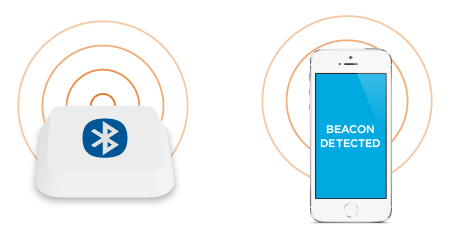
\includegraphics[width=\columnwidth]{beaconPhone}
	\caption{Representación de un beacon emitiendo mediante Bluetooth a un dispositivo móvil}
	\label{fig:beaconBluetooth}
\end{figure}

El funcionamiento de un beacon es sencillo: El beacon emite una señal ininterrumpida que es captada por los dispositivos móviles dentro de su radio de cobertura. La señal nos ofrece información que nos sirve para detectar y localizar estos dispositivos. Esta señal es captada por una aplicación previamente instalada en un dispositivo móvil que esté programada para recibirla y reaccionar de manera acorde a la información recibida.


Hay que tener en cuenta que esta señal es unilateral: los beacons son capaces de enviar pero no están preparados para recibir. También hay que tener en cuenta, que la mayoría de los beacon actuales en el mercado transmiten información preconfigurada, confiando en la aplicacion móvil para utilizar la información; sin embargo es muy posible que esto cambie en un futuro, ampliando las posibilidades de los beacons.

\subsubsection{¿Como funcionan estos dispositivos?}

Los beacons usan Bluetooth Low Energy (BLE) \cite{URL::BluetoothLowEnergy}, una versión del protocolo Bluetooth diseñada para usar mucha menos energía y enviar menos información. Los beacons funcionan con baterías cuyo tiempo de vida depende de la configuración establecida, teniendo en cuenta la emisión de la señal (fuerza y frencuencia) y tiempo de hibernación. Sus tiempos de vida son variables, pudiendo durar desde un mes hasta varios años. 

\begin{figure}[h]
	\centering
	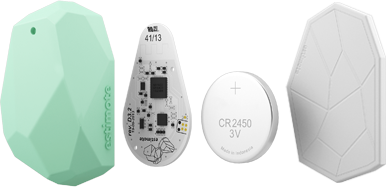
\includegraphics[width=\columnwidth]{estimoteBeaconInside}
	\caption{Interior de un beacon de Estimote}
	\label{fig:beaconInside}
\end{figure}

Independientemente de lo que se pueda pensar, los beacons en sí mismas no transmiten información significativa, transmiten identificadores cortos junto con información customizable breve, que son interpretadas por una aplicación que sabe lo que tiene que hacer con esa información y que es la que se encarga de procesar la información y realizar una acción pertinente.

Este identificador se divide en tres partes: 

\begin{itemize}
\item \textit{''UUID''} \cite{URL::UUID} : corresponde con una ID dada por el vendedor e identifica el beacon en cuestión.
\item ID Superior : customizables y utilizadas con un significado específico que puede identificar una acción o parámetro. 
\item ID Inferior: customizables y utilizadas al igual que la superior con un significado específico que se puede usar para identificar una acción o parámetro.
\end{itemize}

\begin{figure}[h]
	\centering
	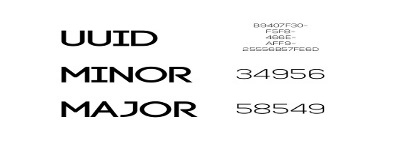
\includegraphics[width=\columnwidth]{identity}
	\caption{Numeros identificativos de los beacons}
	\label{fig:beaconId}
\end{figure}

\subsubsection{¿Qué rango de alcance poseen?}

Actualmente los beacons en el mercado presentan un rango de aproximadamente 70 metros sin obstáculos. Está demostrado que este rango disminuye significativamente al atravesar paredes de metal o ladrillo, otros materiales disminuyen en menor medida el rango. 

Las aplicaciones que trabajan con beacons suelen definir acciones en tres rangos de distancia principalmente: 

\begin{itemize}
\item Lejos: diseñado para que el dispositivo móvil pueda lanzar una acción cuando estás en el rango exterior de un beacon, es decir, cuando se entra en el rango del beacon.
\item Cerca: diseñado para que el dispositivo móvil pueda lanzar una acción cuando estás en el rango interior del beacon. 
\item Inmediato: Diseñado para que el dispositivo móvil pueda lanzar una acción cuando te encuentras muy cercano al beacon.
\end{itemize}

\begin{figure}[h]
	\centering
	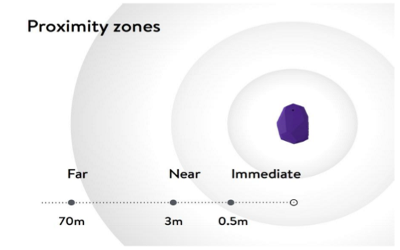
\includegraphics[width=\columnwidth]{BeaconsRange}
	\caption{Ejemplificación del rango de un beacon}
	\label{fig:beaconRange}
\end{figure}

Sin embargo, esto depende de como esté diseñada la aplicación, es posible lanzar acciones a una distancia determinada sin tener en cuenta estos rangos mencionados anteriormente, ya que en todo momento es posible conocer la distancia a la que nos encontramos del beacon.

\subsubsection{¿Con qué dispositivos funcionan?}

Las beacons son compatibles con todos los dispositivos que soporten Bluetooth Low Energy, pero para que las señales de los beacons sean detectadas por tu dispositivo, se ha de tener activado el Bluetooth. 


En dispositivos con IOS7 \cite{URL::IOS7} o superior, el dispositivo puede estar constantemente buscando dispositivos BLE y despertar a las aplicaciones implicadas cuando entran en el rango de los beacons, incluso estando cerradas las aplicaciones.


En dispositivos Android \cite{URL::Android} el sistema operativo no está preparado para escanear dispositivos BLE, por lo que son las aplicaciones las que se tienen que encargar de escanear las proximidades buscando beacons, esto supone que las aplicaciones tienen que estar funcionando, despiertas (aunque sea en segundo plano). Existen librerías que solucionan esta limitación, haciendo que la aplicación escanee cada cierto tiempo incluso en segundo plano o estando dormida, pero no es muy eficaz y suele tener incompatibilidades ya que induce conflictos con el Sistema Operativo. Un ejemplo de estas incompatibilidades lo podemos ver en este hilo de discusión \cite{URL::Incompatibilidades} de los desarrolladores de la librería AltBeacon, librería que se ha usado para BulletPoint y que mencionaremos más tarde.

Por último en dispositivos Windows Phone \cite{URL:WindowsPhone} o Blackberry \cite{URL:Blackberry} existen diferentes niveles de compatibilidad pero en los que soportan BLE, su funcionamiento es similar al de los dispositivos Android, por lo que no nos pararemos a analizarlo. 

\subsubsection{¿Qué ventajas y desventajas tienen con respecto a otras tecnologías?}

A la hora de hablar de los beacons existen una serie de ventajas pero también podemos encontrar algunas desventajas que iremos detallando a continuación. 

Las principales ventajas que se distinguen a la hora de hablar de los beacons son las siguientes: 

\begin{itemize}
\item A diferencia de la tecnología GPS, la activación del bluetooth consume mucho menos batería. 
\item Es una tecnología que puede ser dependiente de la red de datos. 
\item A diferencia de la tecnología GPS, sigue funcionando con precisión en el interior de los edificios.
\end{itemize}

En cuanto a las desventajes que nos podemos encontrar destacamos:

\begin{itemize}
\item Dependen de aplicaciones instaladas en el dispositivo móvil para funcionar. 
\item Es necesario tener el bluetooth activado, lo que consume batería durante el tiempo que esté activado. 
\item Su utilidad depende de la voluntad de terceros de utilizar estos dispositivos, configurarlos y distribuir las aplicaciones.
\end{itemize}

\subsubsection{¿Qué usos se le ha dado a esta tecnología hasta ahora?}

Por ahora esta tecnología se ha utilizado en ambiente muy diversos y con distintas funcionalidades. De los más conocidos podríamos destacar los siguientes: 

\vspace{5mm}

\textsl{\textbf{{Clevedon School (K-12)}}}

\vspace{2mm}

Este ejemplo es bastante significativo ya que se aplicó en el mismo entorno en el que queremos trabajar, una institución de enseñanza universitaria. Después de desplegar cerca de 1200 iPads  la universidad de Clevedon utilizó esta tecnología junto con su aplicación universitaria ya existente. 

\begin{figure}[H]
	\centering
	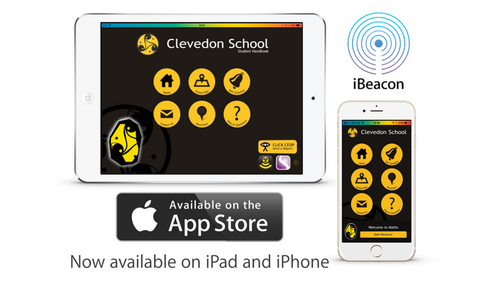
\includegraphics[width=\columnwidth]{ClevedonApp}
	\caption{La aplicación de Clevedon School}
	\label{fig:beaconRange}
\end{figure}


Han sido capaces de crear una manera fácil para que los profesores puedan añadir recursos que se envian automáticamente a los alumnos transitando diferentes zonas en diferentes horarios.Para realizar este trabajo de manera eficiente fue necesario la creación de una Interface para la gestión de los recursos en las diferentes Beacons.


Esta interfaz junto con la aplicación móvil es capaz de: 

\begin{itemize}
\item Programar los recursos para distribuirse a una hora del día especificada. 
\item Programar el material para ser distribuido en un momento determinado durante una clase o evento. 
\item Poner los recursos a disposición de los alumos que se encuentren en una localización específica.
\end{itemize}

Utilizando estos tres recursos, la aplicación, la interfaz y los beacons han sido capaces de crear un entorno interactivo y eficiente motivando tanto a profesores como estudiantes. 

\vspace{5mm}

\textsl{\textbf{{Cleveland Cavaliers Stadium y Levi's Stadium}}}

\vspace{2mm}

Dos de los ejemplos más conocidos han sido los despliegues que se han realizado en estos dos estadios. 

\begin{figure}[H]
	\centering
	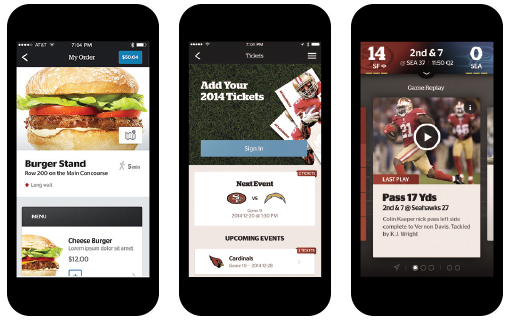
\includegraphics[width=\columnwidth]{LevisStadium}
	\caption{La aplicación de Levi's Stadium}
	\label{fig:levisStadium}
\end{figure}

Por un lado tenemos el despliegue del estadio de Levi's , cuya intención ha sido la de ayudar a sus fans a navegar por el estadio dadas sus dimensiones.En este caso los beacons (de la comañía Aruba Networks) se utilizan en conjunto con puntos de acceso y repetidores situados por toda la infraestructura de manera que queda el estadio cubierto. Con la aplicación los fans también son capaces de ver repeticiones de las jugadas y pedir comida directamente desde sus dispositivos móviles.


Un punto importante de este  despliegue ha sido la monitorización continua del funcionamiento de los beacons, incluyendo si estan en funcionamiento o necesitan bateria nueva. Los beacons son también más económicos que los puntos de acceso WiFi, lo cual les ha beneficiado.

En el caso del estadio de Cleveland, los beacons se encargan de proveer al usuario de información personalizada dependiendo del lugar y la hora. En algunos casos videos, ofertas promocionales y contenido adicional.

\vspace{5mm}

\textsl{\textbf{{Orlando Int'l Airport}}}

\vspace{2mm}

Otro despliegue exitoso de esta tecnología ha sido en el Aeropuerto Internacional de Orlando , donde mediante el uso de los beacons y de una aplicación móvil propia han sido capaces de proporcionar una serie de funcionalidades de vital importancia en una infraestructura como el aeropuerto: 

\begin{itemize}
\item Navegación paso por paso a través de cerca de 1000 establecimientos o servicios dentro del aeropuerto. 
\item Actualizaciones inmediatas de la información de los vuelos. 
\item Intrucciones a puntos de interés criticos como puntos de recogida de equipaje, puertas de embarque o puestos de información.
\end{itemize}

\begin{figure}[H]
	\centering
	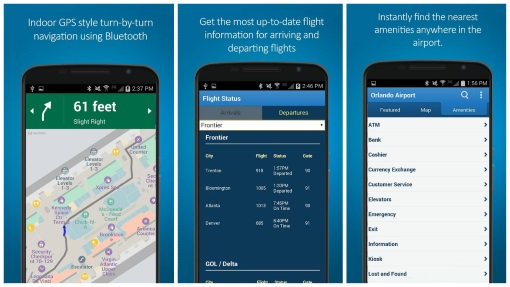
\includegraphics[width=\columnwidth]{orlandoAirport}
	\caption{La aplicación del Aeropuerto Internacional de Orlando}
	\label{fig:orlandoAirport}
\end{figure}

El siguiente punto sería ampliar la opción a los establecimientos de ofrecer anuncios o promociones, opción que mantienen abierta y no se descarta en un futuro.


Esta información ha sido extraída de: \cite{URL::Articulo} 

\subsection{CouchBase Server}

Couchbase Server es una base de datos NoSQL con una arquitectura distribuida orientada al rendimiento, escalabilidad y disponibilidad. Da la oportunidad a los desarrolladores de construir aplicaciones de manera sencilla y rápida combinando la flexibilidad del JSON y la tecnología NoSQL.

\subsubsection{¿Por qué utilizar Couchbase Server?}

Hemos decidido utilizar esta tecnología por su flexibilidad y potencia para almacenar documentos fácilmente. Además resulta muy sencillo integrarla con la tecnología móvil mediante el uso de una base de datos reducida dentro del dispositivo móvil y sincronizándola con la base de datos principal del servidor mediante una puerta de sincronización.

\begin{figure}[H]
	\centering
	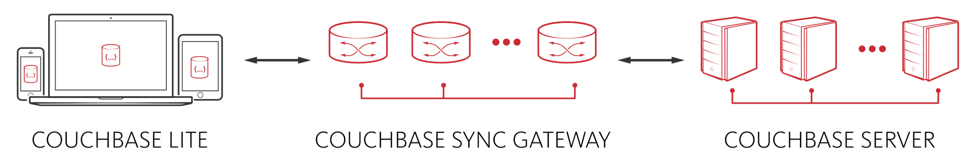
\includegraphics[width=\columnwidth]{couchbaseexplanation}
	\caption{Sincronización de CouchBase Server con CouchBase Lite mediante Sync Gateway}
	\label{fig:couchbaseexplanation}
\end{figure}

En este caso se ha configurado el servidor en un ordenador portátil haciendo uso de las indicaciones de la página web del producto. Se procederá a desglosar brevemente los pasos seguidos a la hora de configurar el servidor.


\subsubsection{Configuración de la arquitectura}

Para configurar el servidor se han seguido los siguientes pasos: 


\begin{itemize}
\item Descargar la versión Community del producto desde la página web siguiendo el enlace: \cite{URL::couchbaseDownload}. 
\item Seguir los pasos de la página de desarrolladores para la instalación y configuración: \cite{URL::couchBaseGuide}. 
\item Una vez configurado CouchBase Server procederemos a descargar Sync Gateway que será el servicio que se encarge de sincronizar el contenido del nuestra aplicación al servidor, para ello lo descargaremos de la página al igual que el servidor siguiendo el link: \cite{URL::couchbaseDownload} .
\item Para vincular el servidor con Sync Gateway es necesario hacer uso de un fichero de configuración con el que lanzaremos el servicio Sync Gateway.
\item Una vez configurado Sync Gateway, ya tenemos el canal de configuración entre el servidor y la aplicación, para utilizar la base de datos móvil seguiremos los pasos desglosados en: \cite{URL::couchBaseLite} .
\end{itemize}


En este caso se ha tenido que conectar el dispositivo al ordenador. Tanto el ordenador como el dispositivo móvil han de estar en la misma red y hemos utilizado la dirección IP de la máquina para realizar las peticiones del móvil al servidor (alojado en el portátil) al utilizar la API. De esta manera se ha comprobado el funcionamiento del servidor, del servicio de sincronización y de la base de datos versión Lite en el dispositivo móvil.


\subsection{La librería AltBeacon}


\subsubsection{¿Qué es AltBeacon?}

Se puede definir AltBeacon como una especificación que: 

\begin{itemize}
\item Define el formato del mensaje publicitario que los beacons transmiten a través de BLE (Bluetooth Low Energy).
\item Intenta crear un mercado abierto y competitivo para implementaciones usando proximidad con los beacons.
\item Puede ser utilizada por todos gratuitamente, sin cuotas ni compromisos.
\item No favorece a ningún proveedor sobre otro. Las limitaciones vienen determinadas por los estándares técnicos del proveedor.
\end{itemize}

A continuación se profundizará en el funcionamiento y configuración de la librería AltBeacon, librería que cumple con la especificación AltBeacon y que se ha utilizado para trabajar en Android.

\subsubsection{Configuración}

Para trabajar con esta librería en Android Studio solo hemos tenido que importarla mediante el uso de Gradle a nuestro proyecto como se explica en : \cite{URL::importGradle}


También es posible descargarla desde la página oficial, donde además podremos econtrar diferentes versiones de la misma, para ello podemos hacer uso del siguiente enlace y seleccionar la versión deseada:  \cite{URL::versionAltBeacon}


\subsubsection{Funcionamiento}

Prácticamente la funcionalidad de esta librería se centra en dos elementos principales: 

\begin{itemize}
\item \textit{''Monitoring''} que sería algo así como supervisar, saber que beacons se encuentran en una región o si ha entrado o salido un beacon de una región.
\item \textit{''Ranging''} que hace referencia a rastrear, permitiendo saber a que distancia se encuentran los beacons en todo momento dentro de una región.
\end{itemize}

Utilizando estas dos funcionalidades la aplicación es capaz de controlar, monitoreando y rastreando los distintos beacons en una determinada región. En la página web de la librería se pueden encontrar ejemplos básicos\cite{URL::altbeaconSamples} de como se realizan estas dos funciones en la sección \textit{''Samples''}, además en la sección \textit{''Documentación''} se pueden encontrar también algunos artículos, que pueden resultar interesantes dependiendo del tipo de aplicación que estes desarrollando.




